
\documentclass[12pt]{amsart}
\usepackage{geometry} % see geometry.pdf on how to lay out the page. There's lots.
\geometry{a4paper} % or letter or a5paper or ... etc
% \geometry{landscape} % rotated page geometry
\usepackage{graphicx} %插入图片的宏包
\usepackage{float} %设置图片浮动位置的宏包
\usepackage{subfigure} %插入多图时用子图显示的宏包
% See the ``Article customise'' template for come common customisations

\title{}
\author{}
\date{} % delete this line to display the current date

%%% BEGIN DOCUMENT
\begin{document}

\begin{figure}[H] %H为当前位置,!htb为忽略美学标准,htbp为浮动图形
\centering %图片居中
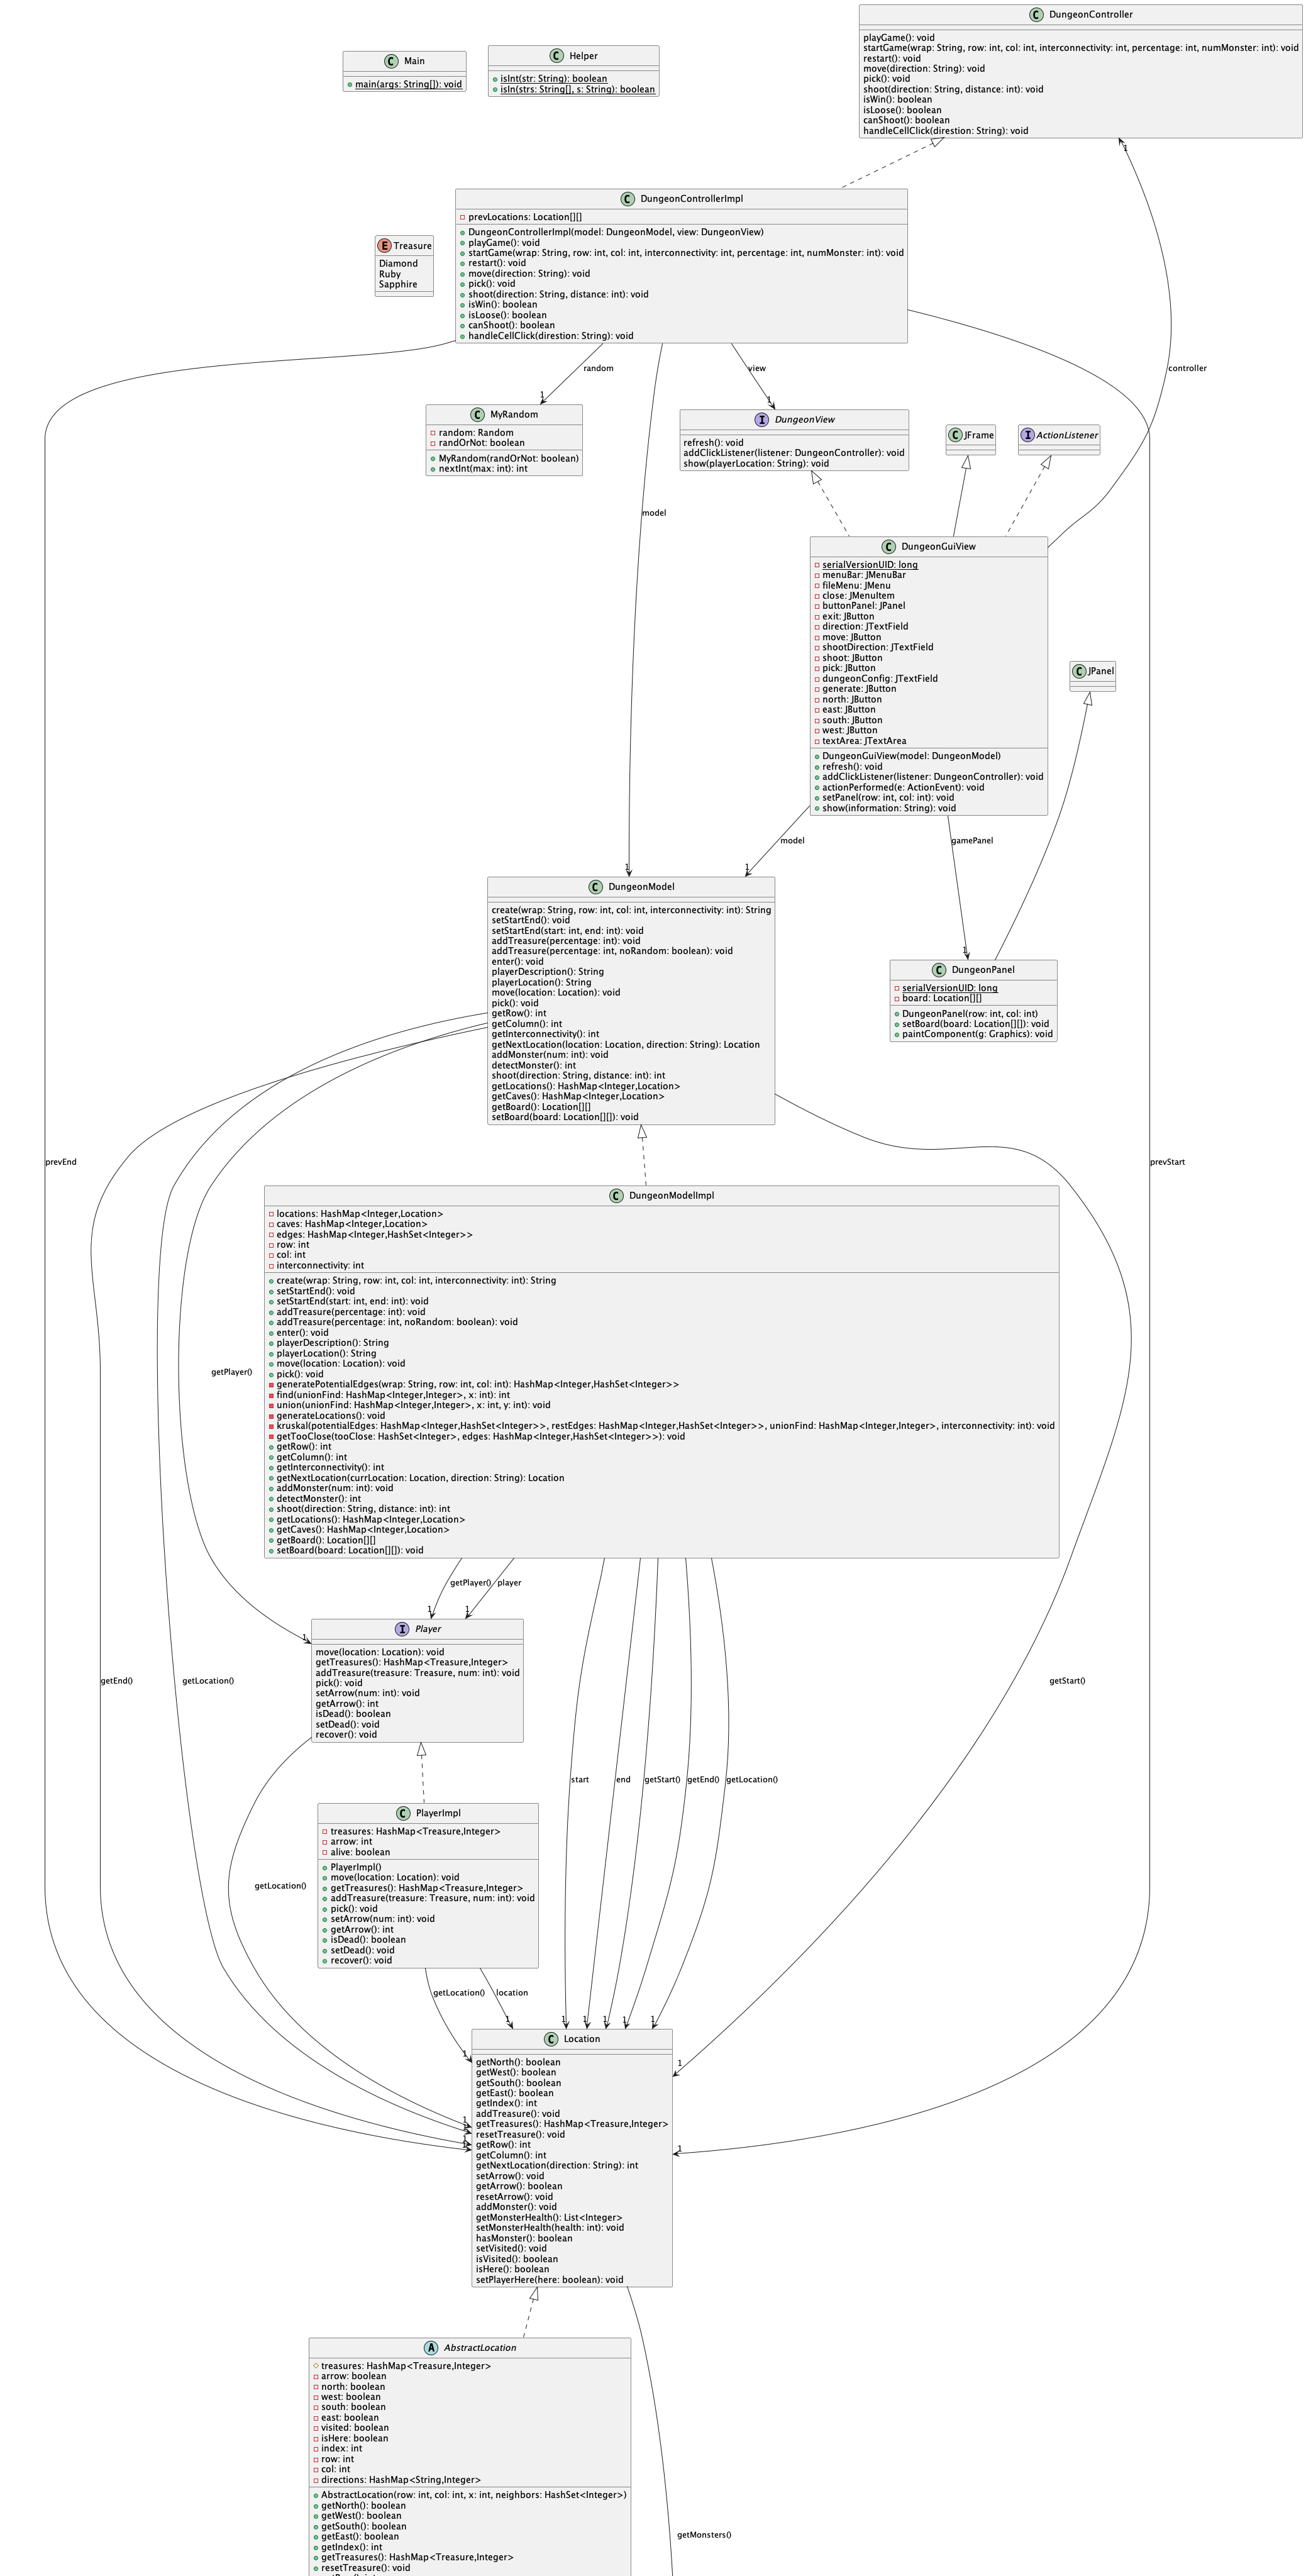
\includegraphics[width=1\textwidth]{uml.png} %插入图片,[]中设置图片大小,{}中是图片文件名
\end{figure}

\newpage

\begin{table}[htbp]
   %\topcaption{Table captions are better up top} % requires the topcapt package
   \begin{tabular}{@{} lll @{}} % Column formatting, @{} suppresses leading/trailing space

      Method     & Input & Expected \\
         controller shoot & Specify direction and distance & Hurt monster if there exists\\
         controller move & String of direction & Controller moves model successfully\\

    \end{tabular}
\end{table}

\newpage

\end{document}



